\cleardoublepage
\newpage
\ThisULCornerWallPaper{1.0}{chapterimage.eps}
\chapter{Zorra}

%Zorra era plomo blanco morochas o chispiado
%Zandor nace 1961 (probablemente)
%%Zandor nace 1961 cuando yo tenía aprox 5-6 años

\begin{wrapfigure}{r}{0.49\textwidth}
  \begin{center}
  \vspace{-30pt}
    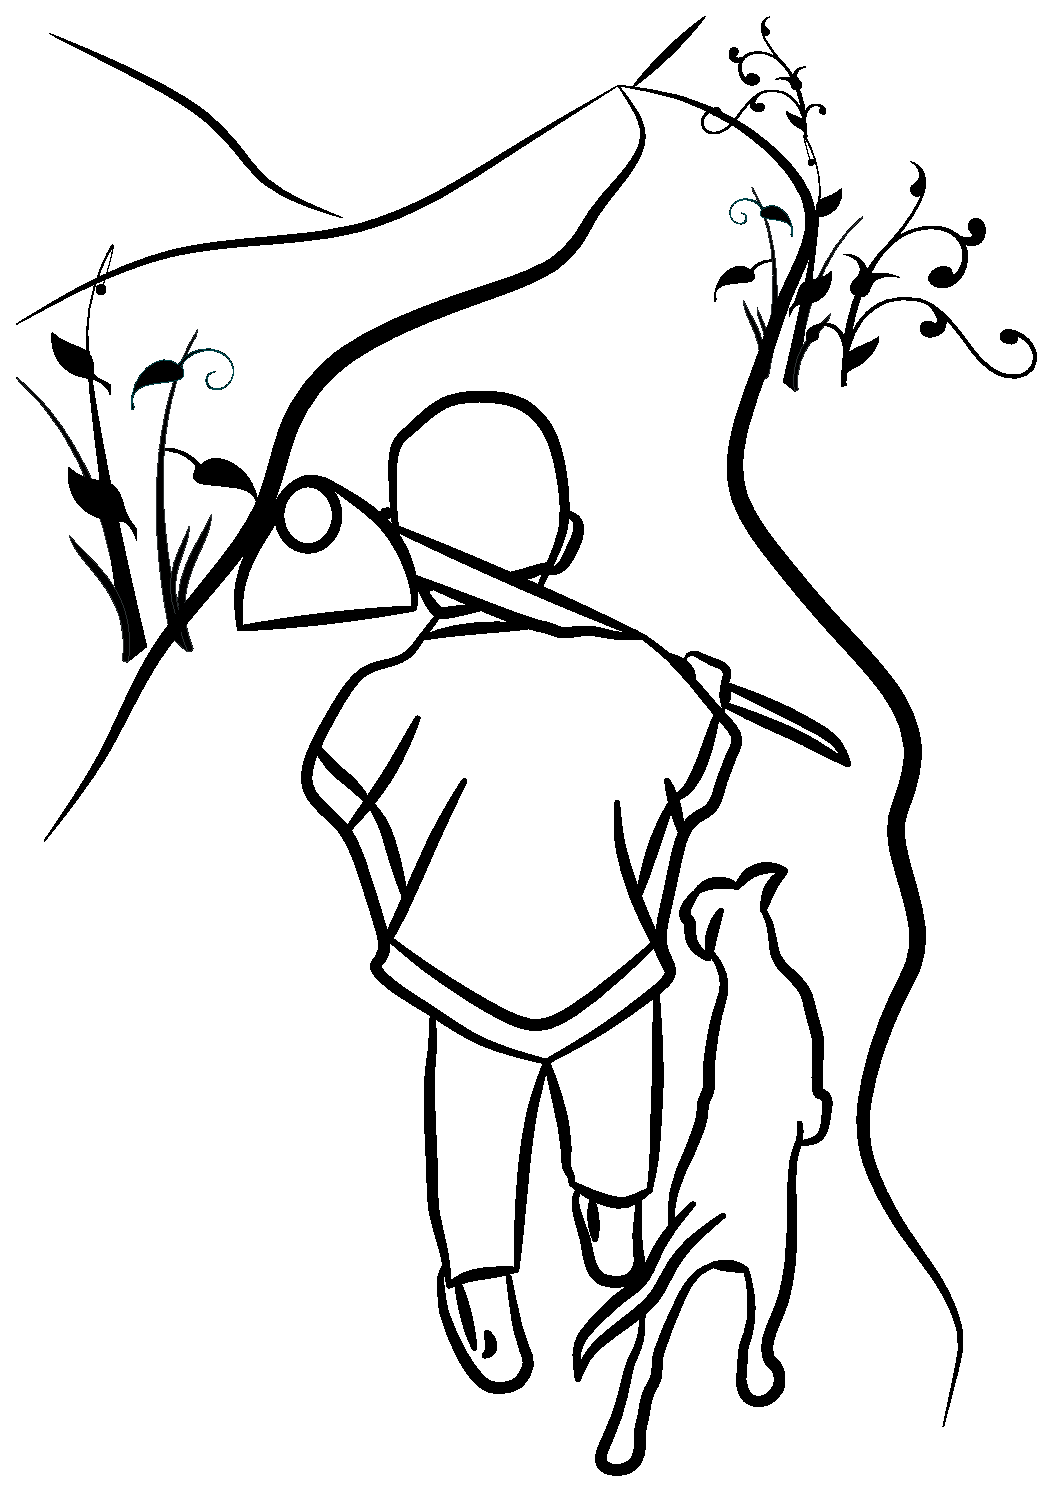
\includegraphics[width=0.47\textwidth]{caminhando.eps}
  \end{center}
  \vspace{-20pt}
  %\caption{Zandor}
\end{wrapfigure}
Quando era criança, minha família tinha uma cadela que se chamava Zorra, ela era de caráter gentil e muito amorosa com todos nós; meu pai e eu gostávamos de andar com ela para todos os lados. Em algumas ocasiões, durante nossas caminhadas, nós avistávamos à distancia a algum conhecido ou familiar, e eles se dirigiam a meu pai falando a viva voz: 
--- Bom dia Don Juande! --- 
Ele respondia entusiasmado essas saudações com a mesma alegria e energia.
Meu pai na verdade se chamava Juan de Dios\footnote{João de Deus}; porém, carinhosamente, todo mundo preferia chamar-lho Don Juande.


Eu provavelmente teria cinco ou seis anos nessa época e lembro de forma clara como minha cadela ia correndo de forma ágil diante de nós, abrindo-nos caminho através dos montes, ladrando e sorrindo.
Estas caminhadas eram muito comuns, uma vez que tínhamos que levar comida para as vacas, procurá-las quando alguma se perdia, ou dar manutenção à chacra.
No princípio eu não tinha percebido que minha cadela tinha alguns maus costumes, pois com ela nós convivíamos e andávamos de dia e seu comportamento era irrepreensível. 

\begin{wrapfigure}{r}{0.42\textwidth}
  \begin{center}
  \vspace{-30pt}
    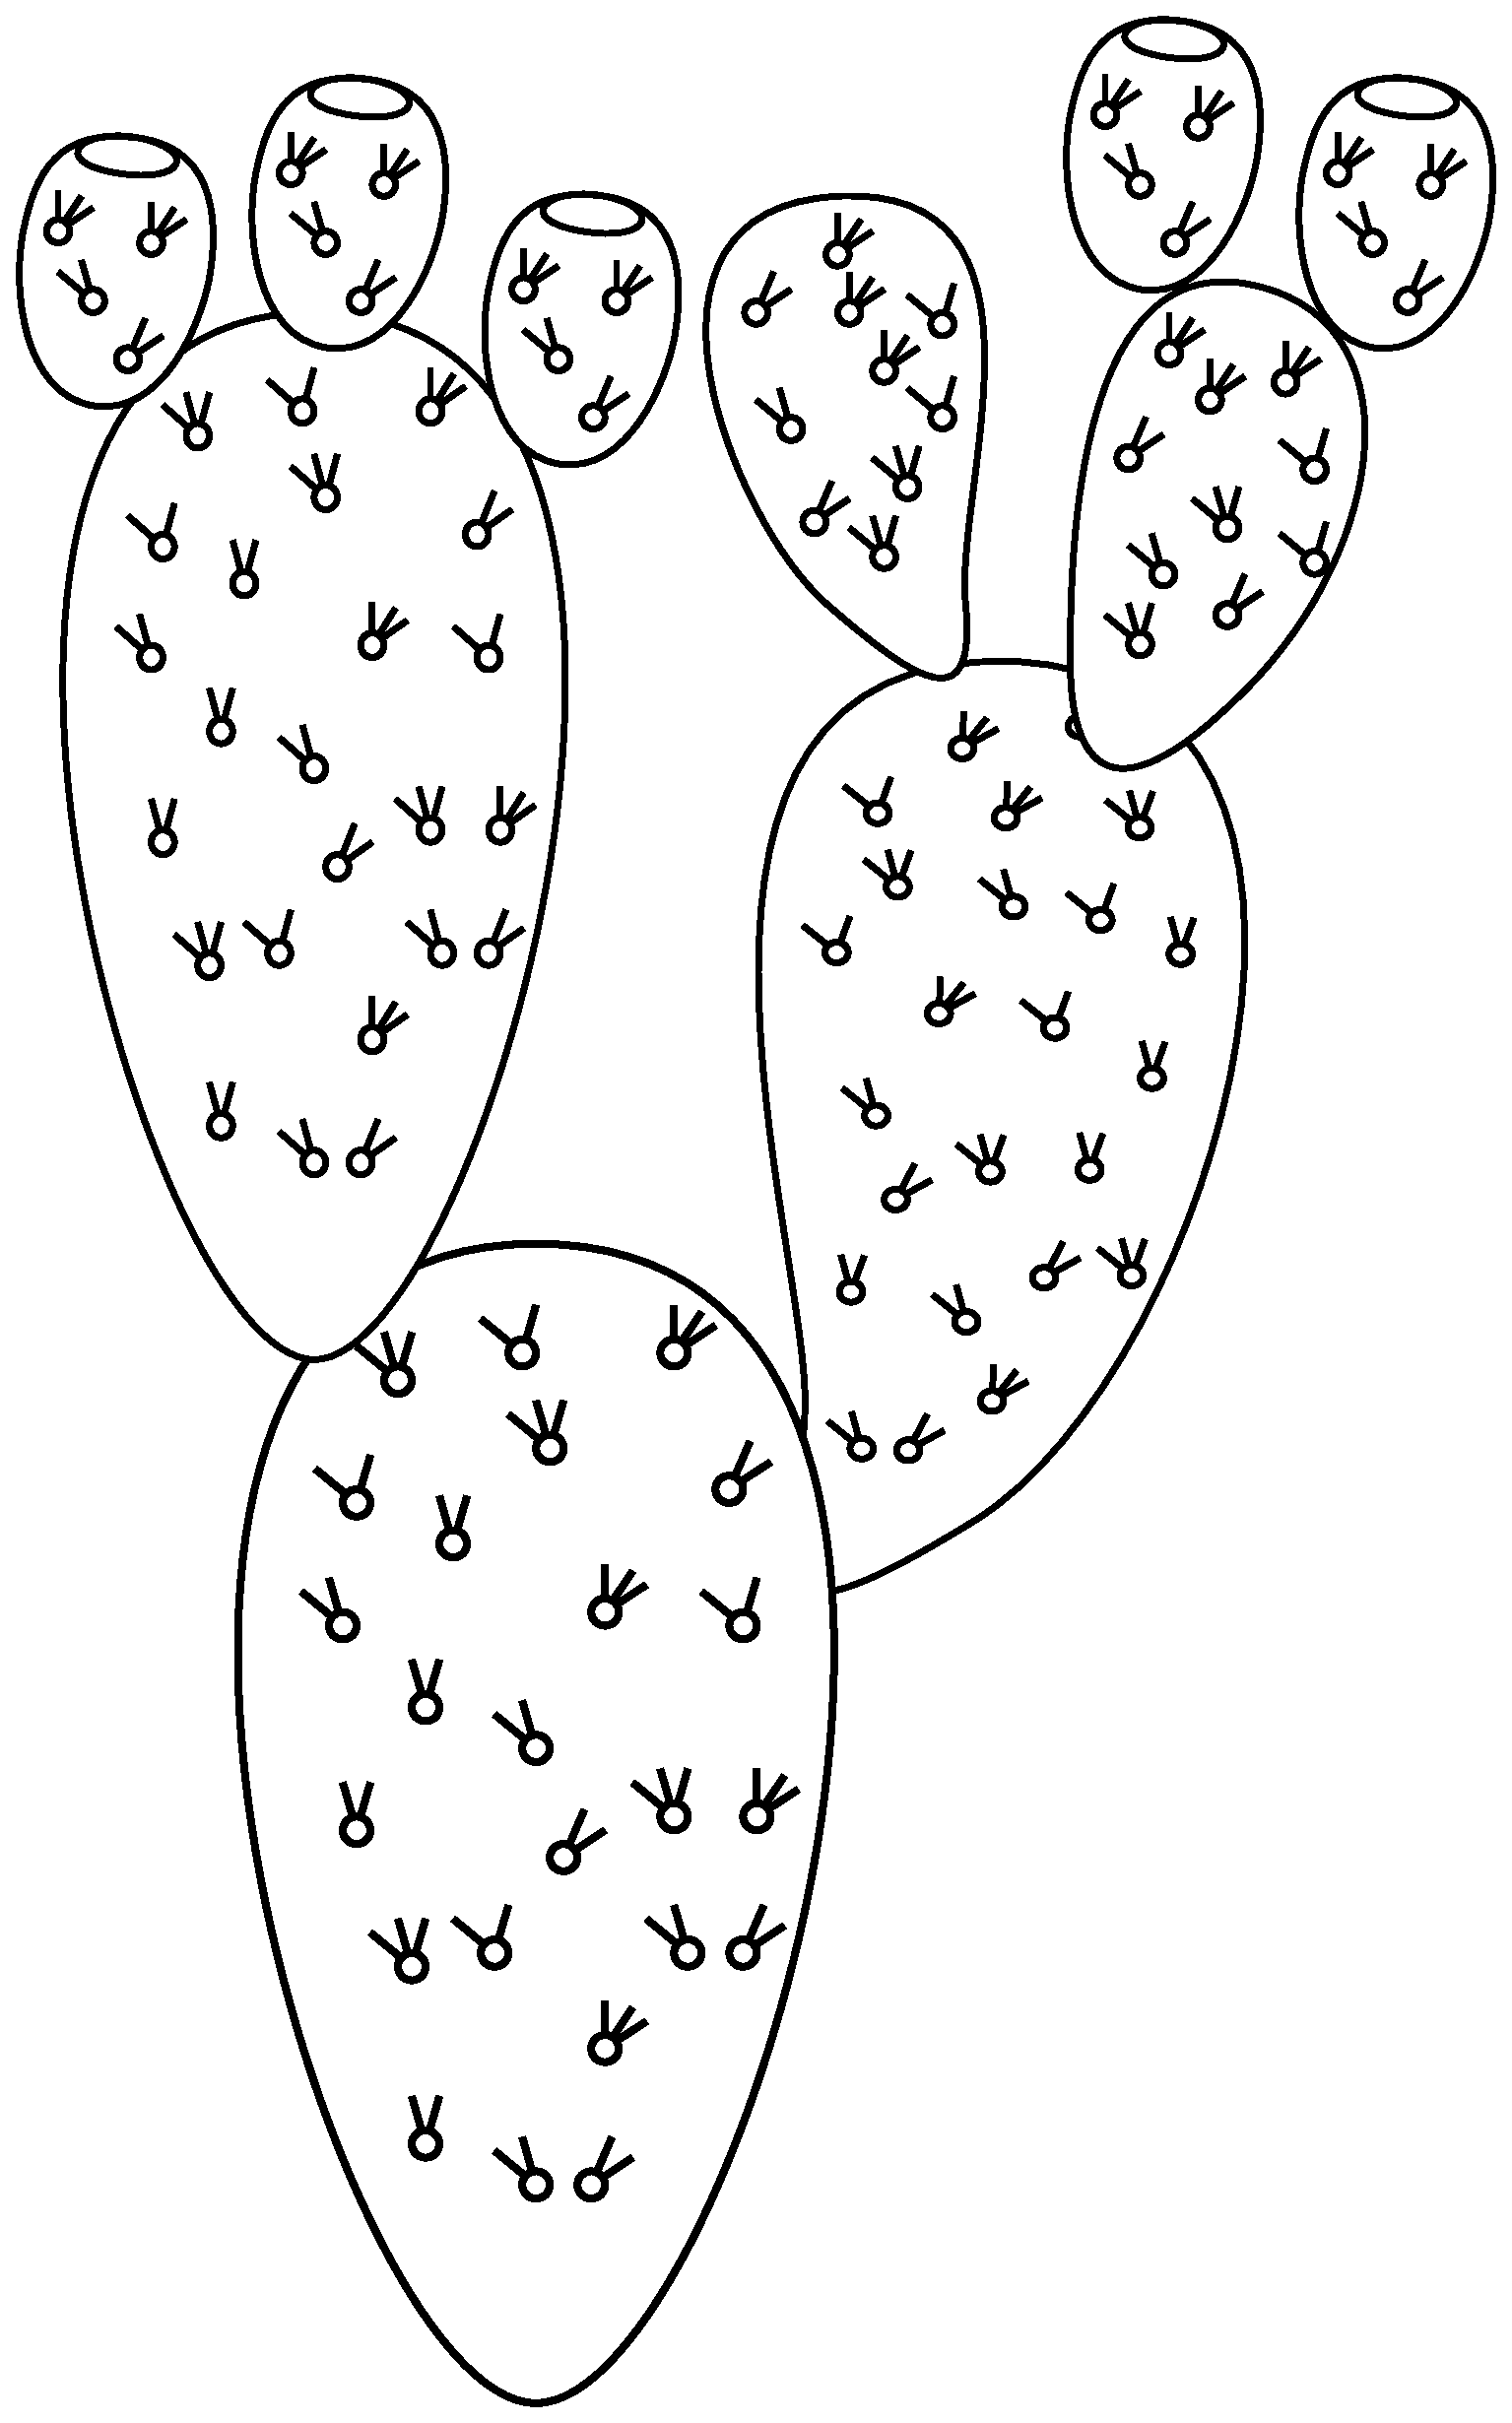
\includegraphics[width=0.4\textwidth]{opuntia.eps}
  \end{center}
  \vspace{-20pt}
  %\caption{Figo das índias.}
\end{wrapfigure}
Ainda lembro a primeira vez que fui ao rio acompanhando meu pai e Zorra; minha mãe tinha encarregado a ele, com caráter de urgência, a missão de obter alguns peixes para serem fritos no almoço; eu rapidamente me uni a tão nobre encomenda, pois gostava de sair a andar. 
Para chegar ao rio, nós tivemos que descer uma ladeira através de um caminho cercado de plantas de figos-da-índia. Quando chegamos lá, eu vi que as margens das águas estavam cheias de juncos, sendo esse um lugar ótimo para explorar e brincar; assim, enquanto meu pai pescava, minha cadela e eu procurávamos ninhos com ovos de perdiz, sem embargo, Zorra sempre os achava primeiro, comia tudo, ou quase tudo, e eu só podia salvar alguns para mim.


Dessa forma passaram alguns anos, nos quais ninguém chegou a nossa casa trazendo alguma reclamação ou comentário sobre Zorra; porém um dia entrei à horta que estava próxima à casa e fiquei surpreendido ao achar vários pequenos ``tesouros'' dentro de um esconderijo. Havia uma sacola de tecido com pão, outra com açúcar, uma com doces e algumas pequenas ferramentas espalhadas. 
Para mim tudo isso era inacreditável, pois nós só tínhamos coisas como açúcar ou bolachas quando meu pai voltava de suas viagens após trabalhar quatro meses em Ica ou alguma outra cidade grande.
Num primeiro momento, a alegria invadiu meu coração, não obstante, lembrei que meu pai era uma pessoa muito rigorosa, não gostava pegar as coisas dos outros, e dizia: 
--- Se você encontra alguma coisa no caminho, no campo, ou na pampa, você não deve pegar, --- 
e ele agregava: 
--- Seguramente alguém o deixou cair, a pessoa que perdeu vai voltar a procurar, e se você leva, ela não vai encontrar.

Eu lembrava muito bem desse ensinamento, porque uma vez, quando estava na solidão do campo pastando as minhas vacas, achei uma ferramenta para fazer fios de lã, que no meu povoado chamávamos de ``callapa''\footnote{Também chamado fuso, este é um utensílio cilíndrico feito geralmente de madeira, utilizado para fiação e torção de fibras como lã.}; provavelmente a ferramenta era de algum outro pastor que passou por ali, mas nesse momento não pensei nisso, só peguei a callapa e retornei a minha casa; já na tarde, cheguei  muito contente, falando: 
--- Mamãe, papai, olhem o que achei no campo! --- 
Meu pai imediatamente respondeu: 
--- Aqui não tem nada para ser encontrado! Isso é de alguém, alguma pessoa perdeu e ela vá ir a procurar. Anda e deixa isso onde você achou.

\begin{wrapfigure}{r}{0.42\textwidth}
  \begin{center}
  \vspace{-10pt}
    
\includegraphics[width=0.4\textwidth]{tools-spindle.eps}
  \end{center}
  \vspace{-20pt}
  %\caption{Figo das índias.}
\end{wrapfigure}
Nesse momento, um frio desceu desde a ponta da minha cabeça até as pontas dos meus pés, pois já quase eram as seis da tarde, tudo estava obscuro, as poucas luzes eram muito distantes e vinham das casas dos vizinhos --- isto era devido a que lá na serra, nessa época, as famílias moravam em casas que estavam separadas, umas de outras, por uma grande distância, 200, 300, 400 metros e algumas vezes até mais ---, e para finalizar, eu era muito medroso no que se refere a lugares obscuros e onde tinha que ir estava muito longe.

Diante da ordem do meu pai, eu fui correndo e chorando nessa direção, no caminho não podia distinguir as coisas a uns metros de mim, porque a lua era minguante; entretanto, quando estava quase na metade do meu destino e meu caminhar era cada vez mais hesitante, observei as sombras ao meu redor, e numa trilha paralela à minha, entre pedras e árvores grandes, vi a silhueta do meu pai me seguindo às escondidas e a uma distância significativa.
Com essa certeza no meu coração, eu segui meu caminho com um pouco mais de tranquilidade, pois sentia que meu pai estava cuidando de mim; mesmo assim, eu seguia chorando de medo, porque na serra, a noite é densa e absoluta, e os sons do caminho alimentavam facilmente a imaginação de uma criança.
No último terço do caminho, eu decidi ir correndo, já que sentia que não podia aguentar mais essa situação; por fim, cheguei ao meu destino, joguei a callapa no exato lugar onde tinha achado e rapidamente empreendi o caminho de retorno.
Na volta também senti a presença do meu pai a alguns metros de mim, ou pelo menos eu queria acreditar isso. Com essa seguridade cheguei a minha casa em menos tempo do que gastei para ir, no entanto, quando entrei: meu pai estava sentado lá como se nada houvesse acontecido.


Por essa velha experiência, e tendo a certeza da autoria de Zorra, já que esse esconderijo era seu lugar favorito, eu tive muito medo por ela, pois sabia que meu pai não iria gostar que Zorra estivesse pegando as coisas de outras pessoas; pelo que se eu avisava a ele, meu pai iria castigá-la severamente. Por esse motivo decidi não dizer nada sobre minha descoberta, entretanto, tenho que reconhecer que: além do amor a minha cadela, também pesou na minha decisão que o lugar estivesse cheio de açúcar, pão e outras coisas, que para nós, gente da serra, eram luxos. 
Por esse motivo decidi passar por ali antes de ir à escola ou à chacra: para comer bolachas, água com açúcar, ou qualquer outra coisa boa que estivesse por ali. 
Para minha desesperação, um dia Zorra trouxe demasiadas coisas, eu  não podia imaginar de onde pegou tudo isso, já que ela só ``trabalhava'' de noite enquanto todos nós dormíamos. Assim, diante desse aumento na criminalidade que largamente desbordava seu esconderijo, meu pai descobriu toda a situação.
Muito para meu pesar, ele castigou severamente a Zorra, desde minha casa eu só escutei seus lamentos recebendo a punição, pois eu preferi não ver.


Depois dessa experiência, ela deixou de levar as coisas à horta, e o problema parecia resolvido, não obstante, logo descobriríamos que longe da casa, numa pedra grande e obscura, perto da casa de um vizinho, 
Zorra havia reiniciado suas atividades; assim, de dia, diante dos olhos da família, se comportava como uma cadela exemplar. Porém, de noite, ela roubava dos vizinhos as mais variadas coisas.

\begin{wrapfigure}{r}{0.42\textwidth}
  \begin{center}
  \vspace{-10pt}
    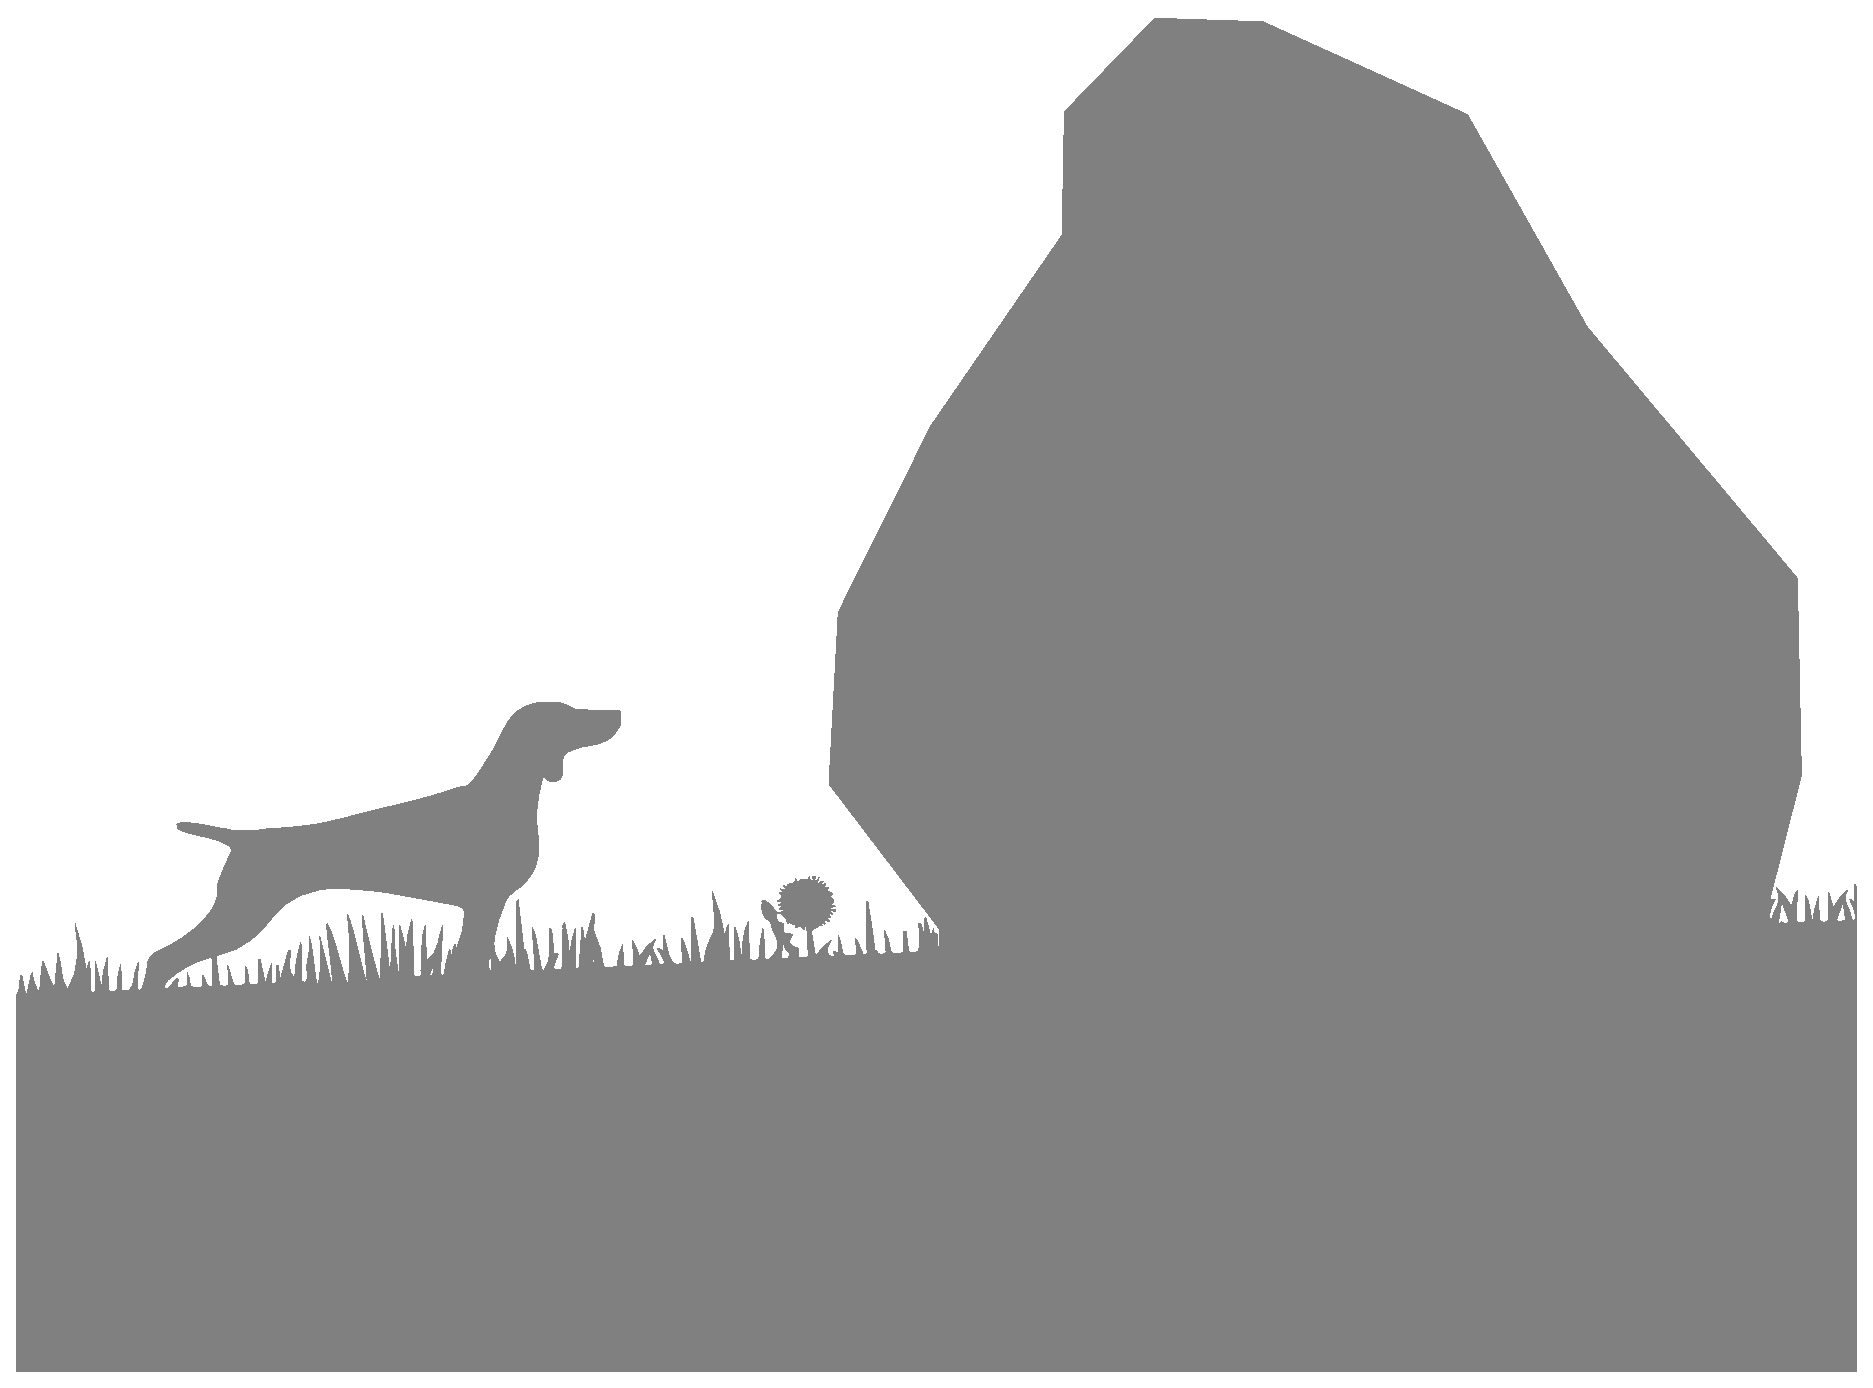
\includegraphics[width=0.4\textwidth]{zorra-rock.eps}
  \end{center}
  \vspace{-20pt}
  %\caption{Figo das índias.}
\end{wrapfigure}
Nesse momento foi a primeira vez que uma pessoa chegou a minha casa para fazer uma reclamação, o pagante denunciou que ele viu em pessoa como Zorra havia entrado na sua casa a roubar. 
A indignação do meu pai foi tão grande quanto sua vergonha, pois não foi um vizinho familiar nosso, que poderia entender a situação, se não que foi uma vítima que morava muito longe de nós, em outro povoado, que foi perguntando entre os vizinhos até achar primeiro suas coisas e logo nossa casa.
Nessa ocasião meu pai castigou mais duramente a Zorra; diante dessa difícil situação, minha maior tristeza era que eu já compreendia que esse problema não ia a solucionar-se com outro castigo, e minhas dúvidas foram confirmadas quando percebi que ela seguia saindo de noite. 

Muito tempo depois descobriríamos que Zorra novamente tinha mudado de esconderijo e que levava suas coisas a outra pedra grande, perto da casa de uma vizinha que era viúva e que carinhosamente chamávamos avó Mesla --- na verdade, ela não era familiar nosso, mas o costume na serra era chamar avó a qualquer pessoa de idade, como sinal de respeito, já que vivíamos com eles como se fossem de nossa família ---.
Assim, antes que alguma pessoa da minha casa conhecesse esse novo lugar, no qual Zorra ocultava seus objetos roubados, outra pessoa chegou a denunciar novamente a cadela, e mesmo que meu pai castigou, gritou e tentou segui-la, não conseguimos achar onde ela escondia as coisas; dessa forma, o tempo transcorreu sem que essa incógnita fosse resolvida. 

Um dia meu pai, minhas irmãs e eu decidimos descer ao rio para pescar, porém esse dia não achamos a Zorra para que nos acompanhasse. Transcorreu o dia e quando eram as quatro ou cinco da tarde, nós estávamos prontos para regressar a casa com a pesca do dia. Nesse momento, eu escutei um ruído entre os juncos do rio, onde costumava brincar com Zorra, por pura curiosidade me acerquei a averiguar que era esse sonido similar a um choro agudo; para minha surpresa, lá estava sozinho um cachorro pequeno e pretinho que minha cadela havia parido.  
Para que meu pai não visse ele, eu escondi o filhote dentro do meu agasalho, já que desconfiava que ele me deixasse levar um novo cachorro a casa, pois os problemas que Zorra gerava já eram suficientes para nós, como para arriscar mais a reputação da família com outro cachorro.
Só quando cheguei em casa tirei o cachorro de dentro das minhas roupas e diante das minhas irmãs, minha mãe e meu pai, apresentei o novo membro da família. Dado que nessa época, minhas irmãs estavam aprendendo a ler usando um livro chamado ``Lola e Pepe'', onde nas suas histórias descreviam a um cachorro chamado Zandor, eu decidi usar esse nome para meu novo cachorro. 

Assim, mesmo com seus novos deveres de mãe, Zorra não deixava de causar problemas, já que aos nossos ouvidos chegavam histórias de roubos em povoados distantes, e as ausências de Zorra se volviam cada vez mais prolongadas.
Para nossa má sorte, num povoado vizinho, tinha-se espalhado a notícia que era uma cadela a responsável de todos os roubos, e, num triste dia, os moradores dessa localidade se organizaram, entre todos encurralaram e atraparam ela e finalmente, sob o abrigo da massa e sem nenhum remorso, deram morte a minha querida Zorra.
Esse mesmo dia chegou na minha casa a notícia da sua morte... entre lágrimas e lamentos fomos a esse povoado a enterrar a nossa querida cadela, já que nos informaram que eles simplesmente tinham jogado seu corpo na beira do rio; quando chegamos lá, a encontramos gelada e inerte, e instintivamente a embrulhamos num tecido, como se fosse um bebê, para que não passasse frio... ao seu lado choramos até que as nossas lágrimas se secaram, pois ela tinha sido nossa amiga fiel, e mesmo que soubéssemos de  seus maus costumes, nós a amávamos.
Nesse mesmo lugar, ao finalizar o dia e com o rio como testemunha, fizemos uma pequena cerimônia e enterramos a quem em vida foi conhecida por nós como Zorra. 

Ao dia seguinte, a notícia tinha se espalhado no meu povoado, e mesmo que nós assumíssemos que não receberíamos condolências de parte dos vizinhos, para nos desenganar, a avó Mesla chegou chorando à porta de nossa casa e entre seus lamentos dizia:
\begin{quotation}
\noindent Eu não tinha panela, e \\Zorra me levou uma panela;\\ 
eu não tinha frigideira, e \\Zorra me levou uma frigideira;\\ 
eu não tinha colher, e \\Zorra me levou uma colher;\\
eu não tinha faca, e \\Zorra me levou uma faca;\\
quando tive fome, \\Zorra me levou pão...  
\end{quotation}
Minha mãe a abraçava, enquanto avó Mesla continuava com sua litania, por aquele animal que, a seu modo de ver, só tinha chegado a sua vida para ajudá-la no seu momento de maior necessidade.
 

